
\chapter{Generalized Operads and Multicategories: Basics}
\lbl{ch:gom-basics}


\chapterquote{%
Three minutes' thought would suffice to find this out; but thought is
irksome and three minutes is a long time}{%
A.E. Houseman}


\noindent
In a category, an arrow has a single object as its domain and a single
object as its codomain.  In a multicategory, an arrow has a finite sequence
of objects as its domain and a single object as its codomain.  What other
things could we have for the domain of an arrow, keeping a single object as
the codomain?  Could we, for instance, have a tree or a many-dimensional
array of objects?  In different terms (logic or computer science): what can
the input%
%
\index{input type}
%
type of an operation be?

In this chapter---the central chapter of the book---we answer these
questions.  We formalize the idea of an input type, and for each input type
we define a corresponding theory of operads and multicategories.  For
instance, the input type might be `finite sequences', and this yields the
theory of ordinary operads and multicategories.  

From now on, operads and multicategories as defined in Chapter~\ref{ch:om}
will be called \demph{plain operads}%
%
\index{operad!plain}%
%
\index{plain}
%
and \demph{plain multicategories}.%
%
\index{multicategory!plain}
%
Some mathematicians are used to their operads coming equipped with
symmetric group actions; they should take `plain' as a pun on `planar', to
remind them that these operads do not.

The formal strategy is as follows.  A small category $C$
can be described as consisting of sets and functions%
%
\index{category!internal}
%
\[
\begin{slopeydiag}
	&	&C_1	&	&	\\
	&\ldTo<\dom&	&\rdTo>\cod&	\\
C_0	&	&	&	&C_0
\end{slopeydiag}
\diagspace
\begin{array}{c}
C_1 \times_{C_0} C_1 \goby{\comp} C_1,	\\
\\
C_0 \goby{\ids} C_1
\end{array}
\]
satisfying associativity and identity axioms, which can be interpreted as
commutative diagrams in \Set.  Here $C_1 \times_{C_0} C_1$ is a certain
pullback, as explained on p.~\pageref{p:defn-caty-pb}.  Similarly, let $T:
\Set \go \Set$ be the functor sending a set $A$ to the underlying set
$\coprod_{n\in\nat} A^n$ of the free monoid on $A$: then a multicategory
can be described as consisting of sets and functions
\[
\begin{slopeydiag}
	& &C_1 & & \\ &\ldTo<\dom& &\rdTo>\cod& \\ TC_0 & & & &C_0
\end{slopeydiag}
\diagspace
\begin{array}{c}
C_1 \times_{TC_0} TC_1 \goby{\comp} C_1,\\
\\
C_0 \goby{\ids} C_1
\end{array}
\]
satisfying associativity and identity axioms (expressed using the monad
structure on $T$).  Here $C_0$ is the set of all objects, $C_1$ is the set
of all arrows, $\dom$ assigns to an arrow the sequence of objects that is
its domain, and $\cod$ assigns to an arrow the single object that is its
codomain.  The crucial point is that this formalism works for any monad $T$
on any category $\Eee$, as long as $\Eee$ and $T$ satisfy some simple
conditions concerning pullbacks.  This gives a definition of
$T$-multicategory for any such $\Eee$ and $T$; in the terms above, the
pair $(\Eee,T)$ is the `input type'.  So when $T$ is the identity monad on
$\Set$, a $T$-multicategory is an ordinary category, and when $T$ is the
free-monoid monad on $\Set$, a $T$-multicategory is a plain multicategory.

We also define $T$-operads.  As in the plain case, these are simply
 $T$-multicategories $C$ with only one object---or formally, those in which
 $C_0$ is a terminal object of $\Eee$.

There is a canonical notion of an algebra for a $T$-multicategory.  Like
their plain counterparts, generalized operads and multicategories can be
regarded as algebraic theories%
%
\index{algebraic theory!generalized multicategory as}
%
(single- and multi-sorted, respectively);
algebras are the accompanying notion of model.  

We start~(\ref{sec:cart-monads}) by describing the simple conditions on
$\Eee$ and $T$ needed to make the definitions work.  Next~(\ref{sec:om})
are the definitions of $T$-multicategory and $T$-operad, and
then~(\ref{sec:algs}) the definition of algebra for a $T$-multicategory (or
$T$-operad).  There are many examples throughout, but some of the most
important ones are done only very briefly; we do them in detail in later
chapters.




\section{Cartesian monads}
\lbl{sec:cart-monads}

In this section we introduce the conditions required of a monad
$(T,\mu,\eta)$ on a category $\Eee$ in order that we may define the notions
of $T$-multicategory and $T$-operad.
% 
\begin{defn}	\lbl{defn:cartesian}
\begin{enumerate}
\item A category $\Eee$ is \demph{cartesian}%
%
\index{category!cartesian}%
%
\index{cartesian}
%
if it has all pullbacks.
\item A functor $\Eee \goby{T} \cat{F}$ is \demph{cartesian}%
%
\index{functor!cartesian}
%
if it preserves
pullbacks. 
\item 	\lbl{part:cart-transf}
A natural transformation $\Eee \ctwo{S}{T}{\alpha} \cat{F}$ is
\demph{cartesian}%
%
\index{transformation!cartesian}
%
if for each map $A \goby{f} B$ in $\Eee$, the naturality
square
%
\begin{diagram}[size=2em]
SA		&\rTo^{Sf}	&SB		\\
\dTo<{\alpha_A}	&		&\dTo>{\alpha_B}\\
TA		&\rTo_{Tf}	&TB		\\
\end{diagram}
%
is a pullback.
\item A monad $(T, T^2\goby{\mu}T, 1\goby{\eta}T)$%
% 
\glo{Tmonad}
% 
on a category $\Eee$ is
\demph{cartesian}%
%
\index{monad!cartesian}
%
if the category $\Eee$, the functor $T$, and the natural
transformations $\mu$ and $\eta$ are all cartesian.
\end{enumerate}
\end{defn}

\begin{remarks}{rmks:cart-defns}
\item All of our examples of cartesian categories will have a terminal%
%
\index{terminal object}
%
object, hence all finite limits.
\item When the category $\cat{E}$ has a terminal object, a (necessary and)
sufficient condition for the natural transformation $\alpha$
of~\bref{part:cart-transf} to be cartesian is that for each object $A$ of
$\Eee$, the naturality square for the unique map $A \go 1$ is a pullback.  
\item Cartesian categories, cartesian functors and cartesian natural
transformations form a sub-2-category \fcat{CartCat} of \Cat, and a
cartesian monad is exactly a monad in \fcat{CartCat}.  (See
p.~\pageref{p:defn-monad-in-bicaty} for the definition of monad in a
2-category.)
\item As is customary, we often write $T$ to mean the whole monad
$(T,\mu,\eta)$. 
\end{remarks}

The rest of the section is examples.

\begin{example}
The identity monad on a cartesian category is cartesian.
\end{example}

\begin{example}		\lbl{eg:mon-monoids}
Let $\Eee = \Set$ and let $T$ be the free-monoid%
%
\index{monoid!free}
%
monad on \Eee.  Certainly
$\Eee$ is cartesian.  An easy calculation shows that the monad $T$ is
cartesian too: Leinster~\cite[1.4(ii)]{GOM}.
\end{example}

\begin{example}		\lbl{eg:comm-not-cart} 
A non-example.  Let $\Eee=\Set$ and let $(T, \mu, \eta)$ be the free
commutative%
%
\index{monoid!commutative!free}
%
monoid monad.  This fails to be cartesian on two counts: $\mu$
is not cartesian (for instance, its naturality square at the unique map
$2\go 1$ is not a pullback), and the functor $T$ does not preserve
pullbacks.  Let us show the latter in detail, using an argument of
Weber~\cite[2.7.2]{Web}.%
%
\index{Weber, Mark}
%
 First note that for any set $A$,
\[
TA = \coprod_{n\in\nat} A^n / S_n
\]
where $S_n$ is the $n$th symmetric group acting on $A^n$ in the natural
way.  Write $[a_1, \ldots, a_n]$ for the equivalence class of $(a_1,
\ldots, a_n) \in A^n$ under this action, so that $[a_1, \ldots, a_n] =
[b_1, \ldots, b_n]$ if and only if there exists $\sigma \in S_n$ such that
$b_i = a_{\sigma i}$ for all $i$.  Now let $x, x', y, y', z$ be distinct
formal symbols and consider applying $T$ to the pullback square
\[
\begin{diagram}[size=2em]
\{(x,y), (x,y'), (x,y'), (x',y')\}	&\rTo	&\{y,y'\}	\\
\dTo					&	&\dTo		\\
\{x,x'\}				&\rTo	&\{z\}.		\\
\end{diagram}
\]
There are distinct elements
\[
[(x,y), (x',y')],
\diagspace
[(x,y'), (x',y)]
\]
of $T \{(x,y), (x,y'), (x,y'), (x',y')\}$, yet both map to $[x,x']
\in T\{x,x'\}$ and to $[y,y'] \in T\{y,y'\}$.  Hence the image of the
square under $T$ is not a pullback.
\end{example}

\begin{example}		\lbl{eg:mon-CJ}%
%
\index{algebraic theory|(}%
%
\index{strongly regular theory|(}
%
Any algebraic theory gives rise to a monad on $\Set$ (its free algebra
monad), and if the theory is strongly regular in the sense
of~\ref{eg:opd-sr} then the monad is cartesian.  Carboni and Johnstone
proved this first~\cite{CJ}; an alternative proof is in
Appendix~\ref{app:special-cart}.  The result implies that the free monoid
monad~(\ref{eg:mon-monoids}) is cartesian, and, as suspected
in~\ref{eg:opd-sr}, that the theory of commutative
monoids~(\ref{eg:comm-not-cart}) is not strongly regular.  Further examples
appear below.
\end{example}

\begin{example}	\lbl{eg:mon-mon-with-inv}
Let $\Eee=\Set$ and let $T$ be the monad corresponding to the theory of
monoids with involution.  By definition, a \demph{monoid with involution}%
%
\index{monoid!involution@with involution}
%
is a monoid equipped with an endomorphism whose composite with itself is
the identity; so this theory is defined by the usual operations and
equations for the theory of monoids together with a unary operation
$\blank^\circ$ satisfying
\[
x^{\circ\circ} = x,
\diagspace
(x\cdot y)^\circ = x^\circ \cdot y^\circ, 
\diagspace
1^\circ = 1.
\]
These equations are strongly regular, so the monad $T$ is cartesian.  Any
abelian group has an underlying monoid with involution, given by $x^\circ =
x^{-1}$.   
\end{example}

\begin{example}		\lbl{eg:mon-mon-with-anti-inv}
More interestingly, let $\Eee=\Set$ and let $T$ be the monad for
\demph{monoids with anti-involution},%
%
\index{monoid!anti-involution@with anti-involution}
%
where an anti-involution on a monoid
is a unary operation $\blank^\circ$ satisfying
\[
x^{\circ\circ} = x,
\diagspace
(x\cdot y)^\circ = y^\circ \cdot x^\circ, 
\diagspace
1^\circ = 1.
\]
Any group whatsoever has an underlying monoid with anti-involution, again
given by $x^\circ = x^{-1}$.  Now, this is \emph{not} a strongly regular
presentation of the theory, and in fact there is no strongly regular
presentation, but $T$ \emph{is} a cartesian monad.  So not all cartesian
monads on $\Set$ arise from strongly regular theories.  These assertions
are proved in Example~\ref{eg:fam-rep-not-opdc}; that $T$ is cartesian was
pointed out to me by Peter Johnstone.%
%
\index{Johnstone, Peter}
%
\end{example}

\begin{example}		\lbl{eg:mon-exceptions}
Let $\Eee = \Set$ and fix a set $S$.  The endofunctor $S + \dashbk$%
%
\index{coproduct!monad from}
%
on
$\Eee$ has a natural monad structure, and the monad is cartesian, corresponding
to the algebraic theory consisting only of one constant for each member of
$S$.  In particular, if $S=1$ then this is the theory of pointed sets.
\end{example}

\begin{example}		\lbl{eg:mon-action}%
%
\index{monoid!action of}%
%
\index{action!monoid@of monoid}
%
Algebraic theories generated by just unary operations correspond to monads
on \Set\ of the form $M\times\dashbk$, where $M$ is a monoid and the unit
and multiplication of the monad are given by those of the monoid.  Since
any equation formed from unary operations and a single variable is strongly
regular, the monad $M\times\dashbk$ on \Set\ is always cartesian.
\end{example}

\begin{example}		\lbl{eg:mon-free-cl-opd}%
%
\index{operad!free}
%
Let $\Eee = \Set^\nat$ and let $T$ be the monad `free plain operad' on
$\Eee$.  As we saw in~\ref{sec:om-further}, the functor $T$ forms trees%
%
\index{tree!vertices labelled@with vertices labelled}
%
with labelled vertices: for instance, if $A \in \Eee$, $a_1 \in A(3)$,
$a_2 \in A(1)$, and $a_3 \in A(2)$, then
\[
% \drmk{tree corr to tensor product }
% \otimes_{a_1}(\otimes_{a_2}(-), -, \otimes_{a_3}(-,-))
\setlength{\unitlength}{1.5em}
\begin{picture}(6,3)(-1.5,0)
% 0th layer
\put(1.5,0){\line(0,1){1}}
% 1st layer
\cell{1.5}{1}{c}{\vx}
\put(1.5,1){\line(-3,2){1.5}}
\put(1.5,1){\line(0,1){1}}
\put(1.5,1){\line(3,2){1.5}}
\cell{0}{2}{c}{\vx}
\cell{3}{2}{c}{\vx}
% top layer
\put(0,2){\line(0,1){1}}
\put(3,2){\line(-1,1){1}}
\put(3,2){\line(1,1){1}}
% labels
\cell{1.8}{1}{tl}{a_1}
\cell{-0.3}{2}{tr}{a_2}
\cell{3.3}{2}{tl}{a_3}
\end{picture}
\]
is an element of $(TA)(4)$.  That $T$ is cartesian follows from theory we
develop later~(\ref{eg:free-cl-opd-cart}).  
\end{example}

\begin{example}		\lbl{eg:mon-tree}
Consider the finitary algebraic theory on $\Set$ generated by one $n$-ary
operation for each $n\in\nat$ and no equations. This theory is strongly
regular, so the induced monad $(T, \mu, \eta)$ on $\Set$ is cartesian.

Given a set $A$, the set $TA$ can be described inductively by
\begin{itemize}
\item if $a\in A$ then $a\in TA$
\item if $t_1, \ldots, t_n \in TA$ then $(t_1, \ldots, t_n) \in TA$.
\end{itemize}
We have already looked at the case $A=1$, where $TA$ is the set of
unlabelled trees~(\ref{eg:opd-of-trees}).  Similarly, an
element of $TA$ can be drawn as a tree%
%
\index{tree!leaves labelled@with leaves labelled}
%
whose leaves are labelled by
elements of $A$: for instance,
\[
((a_1, a_2, ()), a_3, (a_4, a_5)) \in TA
\]
is drawn as
\[
\begin{array}{c}
\setlength{\unitlength}{1.5em}
\begin{picture}(7,4.2)(-0.5,0)
% 0th layer
\put(3,0){\line(0,1){1}}
% 1st layer
\cell{3}{1}{c}{\vx}
\put(3,1){\line(-2,1){2}}
\put(3,1){\line(0,1){1}}
\put(3,1){\line(2,1){2}}
% 2nd layer
\cell{1}{2}{c}{\vx}
\put(1,2){\line(-1,1){1}}
\put(1,2){\line(0,1){1}}
\put(1,2){\line(1,1){1}}
\cell{5}{2}{c}{\vx}
\put(5,2){\line(-1,1){1}}
\put(5,2){\line(1,1){1}}
% invisible top layer
\cell{2}{3}{c}{\vx}
% labels
\cell{0}{3.2}{b}{a_1}
\cell{1}{3.2}{b}{a_2}
\cell{3}{2.2}{b}{a_3}
\cell{4}{3.2}{b}{a_4}
\cell{6}{3.2}{b}{a_5}
\end{picture}
\end{array}.
\]
(Contrast this with the previous example, where the \emph{vertices} were
labelled.)  The unit $A\go TA$ is 
\[
a 
\goesto
\begin{array}{c}
\setlength{\unitlength}{1.5em}
\begin{picture}(1,1.6)(-0.5,0)
\put(0,0){\line(0,1){1}}
\cell{0}{1.2}{b}{a}
\end{picture}
\end{array},
\]
and multiplication $T^2 A \go TA$ takes a tree whose leaves are labelled by
elements of $TA$ (for instance,
\[
\begin{array}{c}
\setlength{\unitlength}{1.5em}
\begin{picture}(4,3.7)(-0.5,0)
% 0th layer
\put(2,0){\line(0,1){1}}
% 1st layer
\cell{2}{1}{c}{\vx}
\put(2,1){\line(-1,1){1}}
\put(2,1){\line(1,1){1}}
% 2nd layer
\cell{1}{2}{c}{\vx}
\put(1,2){\line(-1,1){1}}
\put(1,2){\line(1,1){1}}
% invisible 3rd layer
\cell{2}{3}{c}{\vx}
% labels
\cell{0}{3.2}{b}{t_1}
\cell{3}{2.2}{b}{t_2}
\end{picture}
\end{array},
\]
where
\[
t_1=
\begin{array}{c}
\setlength{\unitlength}{1.5em}
\begin{picture}(3,3.7)(-0.5,0)
% 0th layer
\put(1,0){\line(0,1){1}}
% 1st layer
\cell{1}{1}{c}{\vx}
\put(1,1){\line(-1,1){1}}
\put(1,1){\line(1,1){1}}
% 2nd layer
\cell{2}{2}{c}{\vx}
\put(2,2){\line(0,1){1}}
% labels
\cell{0}{2.2}{b}{a_1}
\cell{2}{3.2}{b}{a_2}
\end{picture}
\end{array},
% 
\diagspace
% 
t_2=
\begin{array}{c}
\setlength{\unitlength}{1.5em}
\begin{picture}(3,3.7)(-0.5,0)
% 0th layer
\put(1,0){\line(0,1){1}}
% 1st layer
\cell{1}{1}{c}{\vx}
\put(1,1){\line(0,1){1}}
% 2nd layer
\cell{1}{2}{c}{\vx}
\put(1,2){\line(-1,1){1}}
\put(1,2){\line(0,1){1}}
\put(1,2){\line(1,1){1}}
% 3rd layer (invisible)
\cell{1}{3}{c}{\vx}
% labels
\cell{0}{3.2}{b}{a_3}
\cell{2}{3.2}{b}{a_4}
\end{picture}
\end{array}
)
\]
and expands the labels to produce a tree whose leaves are labelled by
elements of $A$ (here,
\[
\begin{array}{c}
\setlength{\unitlength}{1.5em}
\begin{picture}(7,5.7)(-0.5,0)
% 0th layer
\put(3.5,0){\line(0,1){1}}
% 1st layer
\cell{3.5}{1}{c}{\vx}
\put(3.5,1){\line(-3,2){1.5}}
\put(3.5,1){\line(3,2){1.5}}
% 2nd layer
\cell{2}{2}{c}{\vx}
\put(2,2){\line(-1,1){1}}
\put(2,2){\line(1,1){1}}
\cell{5}{2}{c}{\vx}
\put(5,2){\line(0,1){1}}
% 3rd layer
\cell{1}{3}{c}{\vx}
\put(1,3){\line(-1,1){1}}
\put(1,3){\line(1,1){1}}
\cell{3}{3}{c}{\vx}
\cell{5}{3}{c}{\vx}
\put(5,3){\line(-1,1){1}}
\put(5,3){\line(0,1){1}}
\put(5,3){\line(1,1){1}}
% 4th layer
\cell{2}{4}{c}{\vx}
\put(2,4){\line(0,1){1}}
\cell{5}{4}{c}{\vx}
% labels
\cell{0}{4.2}{b}{a_1}
\cell{2}{5.2}{b}{a_2}
\cell{4}{4.2}{b}{a_3}
\cell{6}{4.2}{b}{a_4}
\end{picture}
\end{array}
).
\]
\end{example}

\begin{example}%
%
\index{algebraic theory!free}
%
Similar statements can be made for any free theory.  That is, given any
sequence $(\Sigma(n))_{n\in \nat}$ of sets, the finitary algebraic theory
on \Set\ generated by one $n$-ary operation for each $\sigma \in
\Sigma(n)$, and no equations, is strongly regular, so the induced monad
$(T,\mu,\eta)$ on $\Set$ is cartesian.  (The previous example was the case
$\Sigma(n)=1$ for all $n$.)  Given a set $A$, an element of $TA$ can be
drawn as a tree%
%
\index{tree!leaves and vertices labelled@with leaves and vertices labelled}
%
in which the leaves are labelled by elements of $A$ and the
vertices with $n$ branches coming up out of them are labelled by elements
of $\Sigma(n)$: in other words, as a diagram like the domain or codomain
of~\bref{eq:Sigma-mon-cat-iso} (p.~\pageref{eq:Sigma-mon-cat-iso}).%
%
\index{algebraic theory|)}%
%
\index{strongly regular theory|)}
%
\end{example}

\begin{example}		\lbl{eg:mon-free-topo-monoid}%
%
\index{monoid!topological!free}
%
The monad `free topological monoid' on $\Top$, whose functor part sends a
space $A$ to the disjoint union of cartesian powers
$\coprod_{n\in\nat}A^n$, is cartesian (by direct calculation).
\end{example}

\begin{example}		\lbl{eg:mon-free-str-mon-cat}%
%
\index{monoidal category!strict!free}
%
Similarly, the monad `free strict monoidal category' ($=$ free
monoid) on $\Cat$ is cartesian.  In fact, the free monoid monad on a
category $\Eee$ is always cartesian provided that $\Eee$ satisfies the
(co)limit conditions necessary to ensure that the usual free monoid
construction $A \goesto \coprod_{n\in\nat}A^n$ works in $\Eee$.
\end{example}

\begin{example}		\lbl{eg:mnd-sym-mon}%
%
\index{monoidal category!symmetric!free strict}
%
The monad `free symmetric strict monoidal category' on \Cat\ is also
cartesian, as a (lengthy) direct calculation shows.  If we had taken strict
symmetric monoidal categories instead---in other words, insisted that the
symmetries were strict---then we would just be looking at commutative
monoids in \Cat, and the monad would fail to be cartesian by the argument
of Example~\ref{eg:comm-not-cart}.  So weakening%
%
\index{weakening}%
%
\index{categorification}
%
the equality $x \otimes y
= y\otimes x$ to an isomorphism makes a bad monad good.
\end{example}

\begin{example}		\lbl{eg:fc-mnd}
Let $\scat{H}$ be the category $(0 \parpair{\sigma}{\tau} 1)$, so that
\ftrcat{\scat{H}^\op}{\Set} is the category of directed graphs.%
%
\index{graph!directed}
%
 The
forgetful functor $\Cat \go \ftrcat{\scat{H}^\op}{\Set}$ has a left adjoint
and therefore induces a monad $\fc$%
% 
\glo{fc}
% 
(`free category')%
%
\index{category!free (fc)@free ($\fc$)}
%
on
$\ftrcat{\scat{H}^\op}{\Set}$.  It follows from later
theory~(\ref{eg:fc-cart}) that $\fc$ is cartesian.
\end{example}

\begin{example}		\lbl{eg:glob-mnd}
In Part~\ref{part:n-categories} we consider the free strict
$\omega$-category%
%
\index{omega-category@$\omega$-category!strict!free}
%
monad on the category of globular%
%
\index{globular set}
%
sets, and, for
$n\in\nat$, the free strict $n$-category%
%
\index{n-category@$n$-category!strict!free}
%
monad on the category of
$n$-globular sets.  All of these monads are cartesian.  The previous
example is the case $n=1$.
\end{example}

\begin{example}		\lbl{eg:cubical-mnd}
In~\ref{sec:cl-strict} we looked at strict double%
%
\index{double category!strict!free}
%
categories and, more
generally, at strict $n$-tuple categories.%
%
\index{n-tuple category@$n$-tuple category!strict!free}
%
 In particular, we saw that a
strict $n$-tuple category could be described as a functor $(\scat{H}^n)^\op
\go \Set$ with extra structure, where $\scat{H}$ is as in~\ref{eg:fc-mnd}.
The forgetful functor from the category of strict $n$-tuple categories and
strict maps between them to the functor category
$\ftrcat{(\scat{H}^n)^\op}{\Set}$ has a left adjoint, the adjunction is
monadic, and the induced monad on $\ftrcat{(\scat{H}^n)^\op}{\Set}$ is
cartesian.  This can be shown by a similar method to that used for
strict $n$-categories in Appendix~\ref{app:free-strict}.
\end{example}

Alert readers may have noticed that nearly every one of the above examples 
of a cartesian monad on $\Set$ is, in fact, the free-algebra monad for a
certain plain operad.  This is no coincidence, as we discover
in~\ref{sec:alt-app}.



\section{Operads and multicategories}
\lbl{sec:om}


We now define `$T$-multicategory' and `$T$-operad', for any cartesian monad
$T$ on a cartesian category $\Eee$.  That is, for each such $\Eee$ and $T$
we define a category $T\hyph\Multicat$ of $T$-multicategories and a full
subcategory $T\hyph\Operad$ consisting of the $T$-operads.  In the case
$\Eee=\Set$ and $T=\textrm{(free monoid)}$ these are, respectively,
$\Multicat$ and $\Operad$; in the case $\Eee=\Set$ and $T=\id$ they are
$\Cat$ and $\fcat{Monoid}$.%
% 
\glo{Monoid}
% 

The strategy for making these definitions is as described in the
introduction to this chapter, dressed up a little: instead of handling the
data and axioms for a $T$-multicategory directly, we introduce a bicategory
$\Sp{\Eee}{T}$%
% 
\glo{Sp}
% 
and define a $T$-multicategory as a monad in $\Sp{\Eee}{T}$.
This amounts to the same thing, as we shall see.  (All we are doing is
generalizing the description of a small category as a monad in the
bicategory%
%
\index{bicategory!spans@of spans}%
%
\index{span}
%
of spans: B\'enabou~\cite[5.4.3]{Ben}.)%
%
\index{Benabou, Jean@B\'enabou, Jean}
%

\begin{defn}	\lbl{defn:T-spans} 
For any cartesian monad $(T,\mu,\eta)$ on a cartesian category \Eee, the
bicategory $\Sp{\Eee}{T}$ is defined as follows:
%
\begin{description}
\item[0-cells] are objects $E$ of \Eee
%
\item[1-cells $E \go E'$] are diagrams
%
\begin{slopeydiag}
	&	&M	&	&	\\
	&\ldTo<d&	&\rdTo>c&	\\
TE	&	&	&	&E'	\\
\end{slopeydiag}
%
in \Eee
\item[2-cells $(M,d,c) \go (N,q,p)$] are maps $M \go N$ in $\Eee$ such that
%
\begin{slopeydiag}
	&	&M	&	&	\\
	&\ldTo<d&	&\rdTo>c&	\\
TE	&	&\dTo	&	&E'	\\
	&\luTo<q&	&\ruTo>p&	\\
	&	&N	&	&	\\
\end{slopeydiag}
%
commutes
\item[1-cell composition:] the composite of $1$-cells
\[
\begin{slopeydiag}
	&	&M	&	&	\\
	&\ldTo<{d}&	&\rdTo>{c}&	\\
TE	&	&	&	&E'	\\
\end{slopeydiag}
% 
\diagspace
% 
\begin{slopeydiag}
	&	&M'	&	&	\\
	&\ldTo<{d'}&	&\rdTo>{c'}&	\\
TE'	&	&	&	&E''	\\
\end{slopeydiag}
\]
is given by composing along the upper slopes of the diagram
\[
\begin{slopeydiag}
   &       &   &       &   &       &M'\of M\Spbk& &   &       &   \\
   &       &   &       &   &\ldTo  &      &\rdTo  &   &       &   \\
   &       &   &       &TM &       &      &       &M' &       &   \\
   &       &   &\ldTo<{Td}&&\rdTo>{Tc}&   &\ldTo<{d'}&&\rdTo>{c'}&\\
   &       &T^2 E&     &   &       &TE'   &       &   &       &E''\\
   &\ldTo<{\mu_E}&&    &   &       &      &       &   &       &   \\
TE &       &   &       &   &       &      &       &   &       &   \\
\end{slopeydiag}
\]
in $\Eee$, where the right-angle mark in the top square indicates that the
square is a pullback and we assume from now on that a particular
choice%
%
\index{pullback!choice of}
%
of pullbacks in $\Eee$ has been made

\item[1-cell identities:] the identity on $E$ is
%
\begin{slopeydiag}
	&	&E	&	&	\\
	&\ldTo<{\eta_E}&&\rdTo>{1}&	\\
TE	&	&	&	&E	\\
\end{slopeydiag}
%
\item[2-cell compositions and identities] are defined in the evident way 
%
\item[coherence 2-cells:] the associativity and unit 2-cells are defined
using the universal property of pullback.
\end{description}
\end{defn}

Since the choice of pullbacks in $\Eee$ was arbitrary, it is inevitable
that composition of $1$-cells in $\Sp{\Eee}{T}$ does not obey strict
associativity or unit laws.  That it obeys them up to isomorphism is a
consequence of $T$ being cartesian.  Changing the choice%
%
\index{pullback!choice of}
%
of pullbacks in
$\Eee$ only changes the bicategory $\Sp{\Eee}{T}$ up to isomorphism (in the
category of bicategories and weak functors): see
p.~\pageref{p:change-of-shape-rmks}.

Here is the most important definition in this book.  It is due to
Burroni~\cite{Bur},%
%
\index{Burroni, Albert}
%
and in the form presented here uses the notion of monad
in a bicategory (p.~\pageref{p:defn-monad-in-bicaty}).
% 
\begin{defn}		\lbl{defn:T-multicat}
Let $T$ be a cartesian monad on a cartesian category $\Eee$.  A
\demph{$T$-multicategory}%
%
\index{generalized multicategory}
%
is a monad in the bicategory $\Sp{\Eee}{T}$.
\end{defn}

A $T$-multicategory $C$ therefore consists of a diagram
\[
\begin{slopeydiag}
	&		&C_1		&		&	\\
	&\ldTo<\dom	&		&\rdTo>\cod	&	\\
TC_0	&		&		&		&C_0	\\
\end{slopeydiag}
% 
\glo{C0genmti}\glo{C1genmti}\glo{domgenmti}\glo{codgenmti}
%
\]
in $\Eee$ together with maps 
\[
C_{1}\of C_{1} = C_1 \times_{TC_0} TC_1 \goby{\comp} C_{1},
\diagspace
C_{0} \goby{\ids} C_{1}
\]%
% 
\glo{compgenmti}\glo{idsgenmti}%
% 
satisfying associativity and identity axioms---exactly as promised at the
start of the chapter.

\begin{defn}		\lbl{defn:T-operad}
Let $T$ be a cartesian monad on a cartesian category $\Eee$.  A
\demph{$T$-operad}%
%
\index{generalized operad}
%
is a $T$-multicategory $C$ such that $C_0$ is a terminal
object of $\Eee$.
\end{defn}
%
Just as a $T$-multicategory is a generalized category, a $T$-operad is a
generalized monoid.  Explicitly, a monoid in a category $\Eee$ with finite
limits consists of an object $M$ of $\Eee$
together with maps 
\[
M \times M \goby{\mult} M,
\diagspace
1 \goby{\unit} M
\]
in $\Eee$, satisfying associativity and identity axioms.  Take a cartesian
monad $T$ on $\Eee$: then a $T$-operad consists of an object of
$\Eee$ over $T1$, say $P \goby{d} T1$, together with maps
\[
P \times_{T1} TP \goby{\comp} P,
\diagspace
1 \goby{\ids} P
\]
over $T1$ in $\Eee$, again satisfying associativity and identity axioms.


A map of $T$-multicategories is a map of the underlying `graphs' 
preserving composition and identities, as follows.
% 
\begin{defn}	\lbl{defn:T-graph}
Let $T$ be a cartesian monad on a cartesian category $\Eee$. A
\demph{$T$-graph}%
%
\index{generalized graph ($T$-graph)}%
%
\index{T-graph@$T$-graph}\index{graph!generalized ($T$-)}
%
is a diagram
\[
\begin{slopeydiag}
	&		&C_1		&		&	\\
	&\ldTo<\dom	&		&\rdTo>\cod	&	\\
TC_0	&		&		&		&C_0	\\
\end{slopeydiag}
\]
in $\Eee$ (that is, an endomorphism 1-cell in $\Sp{\Eee}{T}$).  A \demph{map
$C \goby{f} C'$ of $T$-graphs} is a pair $(C_0 \goby{f_0} C'_0,\ 
C_1 \goby{f_1} C'_1)$ of maps in $\Eee$ such that
\[
\begin{slopeydiag}
	&	&C_1	&	&	\\
	&\ldTo	&	&\rdTo	&	\\
TC_{0}	&	&\dTo>{f_1}&	&C_0	\\
\dTo<{Tf_{0}}&	&C'_1&	&\dTo>{f_0}\\
	&\ldTo	&	&\rdTo	&	\\
TC'_0&	&	&	&C'_0\\
\end{slopeydiag}
\]
commutes.  The category of $T$-graphs is written $T\hyph\Graph$.%
% 
\glo{TGraph}
% 
\end{defn}

This definition uses two different notions of a map between objects of
\Eee: on the one hand, genuine maps in \Eee, and on the other, spans ($=$
1-cells of $\Sp{\Eee}{T}$).  In Chapter~\ref{ch:fcm} we will integrate the
objects of $\Eee$ and these two different kinds of map into a single
structure, an `\fc-multicategory'.

\begin{defn}	\lbl{defn:multifunctor}%
%
\index{generalized multicategory!map of}
%
A \demph{map $C \goby{f} C'$ of $T$-multicategories} is a map $f$ of
their underlying graphs such that the diagrams 
%
\[
\begin{diagram}[size=2em]
C_0		&\rTo^{\ids}		&C_1		\\	
\dTo<{f_0}	&			&\dTo>{f_1}	\\
C'_0	&\rTo_{\ids}		&C'_1	\\
\end{diagram}
% 
\diagspace
% 
\begin{diagram}[size=2em]
C_1\of C_1	&\rTo^{\comp}		&C_1		\\
\dTo<{f_1 *f_1}	&			&\dTo>{f_1}	\\
C'_1\of C'_1	&\rTo_{\comp}		&C'_1		\\
\end{diagram}
\]
%
commute, where $f_1 * f_1$ is the evident map induced by two copies of $C_1
\goby{f_1} C'_1$.  The category of $T$-multicategories and maps between
them is written $T\hyph\Multicat$.%
% 
\glo{TMulticat}
% 
 The full subcategory consisting of
$T$-operads is written $T\hyph\Operad$.%
% 
\glo{TOperad}
% 
\end{defn}

So for any cartesian monad $T$, we have categories and functors
\[
T\hyph\Operad \rIncl 
T\hyph\Multicat \goby{\textrm{\footnotesize forgetful}}
T\hyph\Graph.
\]
When the extra clarity is needed, we will refer to $T$-multicategories as
\demph{\Cartpr-multicategories}%
%
\index{ET-multicategory etc.@`$\Cartpr$-multicategory' etc.}
%
and to the category they form as
$\Cartpr\hyph\Multicat$; similarly for operads and graphs. 

We now look at some examples of generalized multicategories.  In many of
the most interesting ones the input of each operation/arrow forms quite a
complicated shape, such as a diagram of pasted-together higher-dimensional
cells.  These examples are only described briefly here, with proper
discussions postponed to later chapters.

We start with the two motivating cases.

\begin{example}
Let $T$ be the identity monad on $\Eee=\Set$.  Then $\Sp{\Eee}{T}$ is what
is usually called the `bicategory%
%
\index{bicategory!spans@of spans}%
%
\index{span}
%
of spans' (B\'enabou~\cite[2.6]{Ben}), and a
monad in $\Sp{\Eee}{T}$ is just a small category.  So
\[
(\Set,\id)\hyph\Multicat 
\eqv
\Cat,
\diagspace
(\Set,\id)\hyph\Operad
\eqv
\fcat{Monoid}.
\]
More generally, if $\Eee$ is any cartesian category then
$(\Eee, \id)$-multicategories are categories%
%
\index{category!internal}
%
in $\Eee$ and
$(\Eee, \id)$-operads are monoids%
%
\index{monoid!monoidal category@in monoidal category}
%
in $\Eee$.
\end{example}

\begin{example}	\lbl{eg:cl-oms-are-gen}%
%
\index{monoid!free}
%
Let $T$ be the free monoid monad on the category $\Eee$ of sets.  A
$T$-graph
\[
TC_0 = \coprod_{n\in\nat}C_0^n \ogby{\dom} C_1 \goby{\cod} C_0
\]
amounts to a set $C_0$ `of objects' together with a set $C(a_1, \ldots,
a_n; a)$ for each $n\geq 0$ and $a_1, \ldots, a_n, a \in C_0$.  
The composite 1-cell
\[
\begin{slopeydiag}
           &         &C_1 \of C_1      &          &           \\
           &\ldTo<{\dom'}&             &\rdTo>{\cod'}&        \\
TC_0       &         &                 &          &C_0        \\
\end{slopeydiag}
\]
in $\Sp{\Eee}{T}$ is as follows: the set $C_1 \of C_1$ at the apex is 
\[
C_1 \times_{TC_0} TC_1	
=	
\coprod_{%
\begin{scriptarray}
\scriptstyle
n, k_1, \ldots, k_n \in\nat,	\\
\scriptstyle
a_i^j, a_i, a \in C_0
\end{scriptarray}}	
\begin{array}[t]{l}
C(a_1, \ldots, a_n; a) \times
C(a_1^1, \ldots, a_1^{k_1}; a_1) \times\cdots
\\
\times C(a_n^1, \ldots, a_n^{k_n}; a_n),
\end{array}
\]
an element of which looks like the left-hand side of
Fig.~\ref{fig:multi-comp} (p.~\pageref{fig:multi-comp}); the function
$\dom'$ sends this element to 
\[
(a_1^1, \ldots, a_1^{k_1}, \ldots, a_n^1, \ldots, a_n^{k_n}) \in TC_0,
\]
and $\cod'$ sends it to $a$.  The identity 1-cell on $C_0$ in
$\Sp{\Eee}{T}$ is 
\[
\begin{slopeydiag}
           &         &C_0           &          &           \\
           &\ldTo<{\eta_{C_0}}&     &\rdTo>{1} &           \\
TC_0       &         &              &          &C_0,       \\
\end{slopeydiag}
\]
and $\eta_{C_0}$ sends $a\in C_0$ to $(a) \in TC_0$.  A
$T$-multicategory structure on a $T$-graph $C$ therefore consists of a
function $\comp$ as in Fig.~\ref{fig:multi-comp} and a function $\ids$
assigning to each object $a\in C_0$ an `identity' element $1_a \in C(a;a)$,
obeying associativity and identity laws.  So a $T$-multicategory is just a
plain%
%
\index{multicategory!generalized multicategory@as generalized multicategory}
%
multicategory; indeed, there are equivalences of categories
\[
T\hyph\Multicat \eqv \Multicat, 
\diagspace
T\hyph\Operad \eqv \Operad.
%
\index{operad!generalized operad@as generalized operad}
%
\]
\end{example}

\begin{example}	\lbl{eg:sym-ops}
Suppose we try to realize symmetric operads~(\ref{defn:sym-mti})%
%
\index{operad!symmetric vs. generalized@symmetric \vs.\ generalized}%
%
\index{multicategory!symmetric vs. generalized@symmetric \vs.\ generalized!multicategory for multicategories}
%
as
$T$-operads for some $T$.  A first attempt might be to take the free
commutative monoid monad $T$ on $\Set$. But this is both misguided and
doomed to failure: misguided because if $P$ is a symmetric operad then the
maps $\dashbk\cdot\sigma: P(n) \go P(n)$ coming from permutations
$\sigma\in S_n$ are only isomorphisms, not%
%
\index{weakening}
%
identities; and doomed to
failure because $T$ is not cartesian~(\ref{eg:comm-not-cart}), which
prevents us from making a definition of $T$-operad---in particular, from
expressing associativity and identity laws.  A better idea is to take the
free symmetric%
%
\index{monoidal category!symmetric!free strict}
%
strict monoidal category monad on $\Cat$, thus replacing
identities by isomorphisms: see~\ref{eg:mti-sym} below.
\end{example}

\begin{example}	\lbl{eg:mti-inv}
Let $\Eee=\Set$ and let $T$ be the free monoid-with-involution%
%
\index{monoid!involution@with involution}
%
monad on
$\Eee$, as in~\ref{eg:mon-mon-with-inv}.  A $T$-multicategory looks
like a plain multicategory except that the arrows are of the form
\[
a_1^{\sigma_1}, \ldots, a_n^{\sigma_n} \go a
\]
where the $a_i$'s and $a$ are objects and $\sigma_i \in \{-1,+1\}$.  (It is
sometimes convenient to write $x^{-1}$ instead of $x^\circ$ and $x^{+1}$
instead of $x$.)  For instance:
%
\begin{enumerate}
\item \lbl{eg:mti-inv-Cat}
There is a large $T$-multicategory $\Cat$%
%
\index{category!generalized multicategory of}
%
whose objects are all
small categories and in which a map
\[
A_1^{\sigma_1}, \ldots, A_n^{\sigma_n} \go A
\]
is a functor 
\[
A_1^{\sigma_1} \times\cdots\times A_n^{\sigma_n} \go A
\]
where 
\[
A_i^{\sigma_i} = 
\left\{
\begin{array}{ll}
A_i^\op	&\textrm{if } \sigma_i = -1	\\
A_i	&\textrm{if } \sigma_i = +1.	\\
\end{array}
\right.
\]
Composition in $\Cat$ is usual composition of functors, taking opposites
where necessary.  That $\Cat$ does form a $T$-multicategory (and not just a
plain multicategory) is a statement about the behaviour of contravariance
with respect to products and functors.  A `calculus of substitution' of
this kind was envisaged by Kelly%
%
\index{Kelly, Max}
%
in the introduction to his~\cite{KelMVFI}
paper. 
% 
\item 	\lbl{eg:mti-inv-gen}
More generally, suppose that $(\cat{A},\otimes,I)$ is a monoidal
category and $\blank^\circ: \cat{A} \go \cat{A}$ a functor for which there
are coherent natural isomorphisms
\[
(A^\circ)^\circ \iso A,
\diagspace
(A \otimes B)^\circ \iso A^\circ \otimes B^\circ,
\diagspace
I^\circ \iso I
\]
($A, B \in \cat{A}$): then we obtain a $T$-multicategory in the same way as
we did for $\Cat$ above.  (Beware that although a typical duality%
%
\index{duality!operator}
%
operator
$\blank^\circ$, such as that for duals of finite-dimensional vector spaces,
does satisfy the three displayed isomorphisms, it is a \emph{contravariant}
functor on $\cat{A}$, so does not give a $T$-multicategory.)
\end{enumerate}
%
\end{example}

\begin{example}	\lbl{eg:mti-anti-inv}%
%
\index{monoid!anti-involution@with anti-involution}
%
Now consider the monad $T$ for monoids with \emph{anti}-involution, as
in~\ref{eg:mon-mon-with-anti-inv}.  $T$-multicategories are the
same as in the previous example except that substitution reverses order.
For instance:
%
\begin{enumerate}
\item Example~\ref{eg:mti-inv}\bref{eg:mti-inv-Cat} is also an example of a
$T$-multicategory for the present $T$, since $A \times B \iso B \times A$
for categories $A$ and $B$.
\item Example~\ref{eg:mti-inv}\bref{eg:mti-inv-gen} can also be repeated,
except that now we require $\blank^\circ$ to reverse, rather than preserve,
the order of the tensored factors:
\[
(A \otimes B)^\circ \iso (B\otimes A)^\circ
\]
naturally in $A, B \in \cat{A}$.  
\item Loop%
%
\index{loop space!generalized multicategory from}
%
spaces give an example.  Fix a space $X$ with a basepoint $x$.
In~\ref{eg:mon-cat-loops} we met the monoidal category $\cat{A}$ whose
objects are loops based at $x$ and whose tensor $\otimes$ is concatenation
of loops.  There is a functor $\blank^\circ: \cat{A} \go \cat{A}$ sending a
loop to the same loop run backwards, and this satisfies
\[
(\gamma^\circ)^\circ = \gamma,
\diagspace
(\gamma \otimes \delta)^\circ = \delta^\circ \otimes \gamma^\circ,
\diagspace
\mr{const}_x^\circ = \mr{const}_x
\]
for all loops $\gamma$ and $\delta$.  So there is a resulting
$T$-multicategory whose objects are loops and whose maps encode all the
information about concatenation of loops, homotopy classes of homotopies
between loops, and reversal%
%
\index{invertibility}
%
of loops.
\end{enumerate}
%
\end{example}

\begin{example}	\lbl{eg:mti-exceptions}
Let $\Eee = \Set$ and let $T$ be the monad $1 + \dashbk$%
%
\index{coproduct!monad from}%
%
\index{pointed set}
%
of~\ref{eg:mon-exceptions}.  A $T$-graph is a diagram $1+C_0 \ogby{\dom}
C_1 \goby{\cod} C_0$ of sets and functions.  If we regard $1 + C_0$ as a
subset of the free monoid $\coprod_{n\in\nat} C_0^n$ on $C_0$ and recall
Example~\ref{eg:cl-oms-are-gen} then it is clear that a $T$-multicategory
is exactly a plain multicategory in which all arrows are either unary or
nullary.  So it is natural to draw an arrow $\theta$ of $C$ as either
\[
\begin{centredpic}
\begin{picture}(8,4)(0,-2)
\cell{2}{0}{r}{\tinputlft{a}}
\cell{2}{0}{l}{\tusual{\theta}}
\cell{6}{0}{l}{\toutputrgt{b}}
\end{picture}
\end{centredpic}
\diagspace
\textrm{or}
\diagspace
\begin{centredpic}
\begin{picture}(6,4)(0,-2)
\cell{0}{0}{l}{\tusual{\theta}}
\cell{4}{0}{l}{\toutputrgt{b}}
\end{picture}
\end{centredpic}
\]
where in the first case $\dom(\theta) = a \in C_0$, in the second
$\dom(\theta)$ is the unique element of $1$, and in both $\cod(\theta) =
b$.  The unary arrows form a category $D$, and the nullary arrows define a
functor $Y: D \go \Set$ in which $Y(b)$ is the set of nullary arrows with
codomain $b$.  So a $T$-multicategory is the same thing as a small category
$D$ together with a functor $Y: D \go \Set$, and in particular, a
$T$-operad is a monoid acting%
%
\index{action!monoid@of monoid}%
%
\index{monoid!action of}
%
on a set.  Similarly, if $S$ is any set then
a $(\Set, S + \dashbk)$-multicategory is a small category $D$ together with
an $S$-indexed family of functors $(D \goby{Y_s} \Set)_{s \in S}$.

Another way of putting this is that, when $T = 1 + \dashbk$, a
$T$-multicategory is a discrete opfibration%
%
\index{fibration!discrete opfibration}
%
(p.~\pageref{p:defn-cl-d-opfib}).  In fact, $T\hyph\Multicat$ is equivalent
to the category whose objects are discrete opfibrations between small
categories and whose morphisms are commutative squares.
\end{example}

\begin{example}	\lbl{eg:semigp-mti}
As a kind of dual to the last example, let $\Eee=\Set$ and let $T$ be the
free semigroup%
%
\index{semigroup!free}
%
monad, $TA = \coprod_{n\geq 1} A^n$.  Then a
$T$-multicategory is exactly a plain multicategory with no nullary%
%
\index{nullary!arrow}
%
arrows.  In particular, a $T$-operad $P$ is a family $(P(n))_{n\geq 1}$ of
sets, indexed over positive numbers, equipped with composition and
identities of the usual kind.  Some authors prefer to exclude the
possibility of nullary operations: see the Notes to Chapter~\ref{ch:om}.
\end{example}

\begin{example}	\lbl{eg:M-times-mti}
Fix a monoid%
%
\index{monoid!action of}%
%
\index{action!monoid@of monoid}
%
$M$ and let $T$ be the monad $M\times\dashbk$ on $\Set$, as
in~\ref{eg:mon-action}.  Then a $T$-graph is a diagram $M\times C_0 \og C_1
\go C_0$, and by projecting onto the two factors of $M \times C_0$ we find
that $T\hyph\Multicat$ is isomorphic to the category $\Cat/M$ of categories
over $M$.  (Here we regard a monoid as a one-object category:
p.~\pageref{p:degen-cat-monoid}.)  In particular, $T\hyph\Operad \iso
\fcat{Monoid}/M$.

For a specific example, let $M$ be the (large) monoid of all cardinals%
%
\index{cardinals}
%
under multiplication.  Let $C$ be the (large) category of fields%
%
\index{fields, category of}
%
and
homomorphisms between them (which are, of course, all injective).  By
taking degrees%
%
\index{degree of extension}
%
of extensions we obtain a functor $\pi: C \go M$, making
fields into an $(M\times\dashbk)$-multicategory.
\end{example}

\begin{example}	\lbl{eg:mti-free-cl-opd}%
%
\index{operad!free}
%
Let $T$ be the free plain operad monad on $\Eee = \Set^\nat$, as
in~\ref{eg:mon-free-cl-opd}.  In a $T$-multicategory the objects form a
graded set $(C_0(n))_{n\in\nat}$ and the arrows look like%
%
\index{tree!vertices labelled@with vertices labelled}
%
\[
\setlength{\unitlength}{1.5em}
\begin{picture}(14.5,3)(0,-1.5)
\cell{0}{0}{l}{%
\begin{picture}(6,3)(-1.5,0)
% 0th layer
\put(1.5,0){\line(0,1){1}}
% 1st layer
\cell{1.5}{1}{c}{\vx}
\put(1.5,1){\line(-3,2){1.5}}
\put(1.5,1){\line(0,1){1}}
\put(1.5,1){\line(3,2){1.5}}
\cell{0}{2}{c}{\vx}
\cell{3}{2}{c}{\vx}
% 2nd layer
\put(0,2){\line(0,1){1}}
\put(3,2){\line(-1,1){1}}
\put(3,2){\line(1,1){1}}
% labels
\cell{1.8}{1}{tl}{a_1}
\cell{-0.3}{2}{tr}{a_2}
\cell{3.3}{2}{tl}{a_3}
\end{picture}}
%
\put(6.5,0){\vector(1,0){3}}
\cell{8}{0.2}{b}{\theta}
%
\cell{10.5}{0}{l}{%
\begin{picture}(4,2)(-2,0)
% lower layer
\put(0,0){\line(0,1){1}}
% upper layer
\cell{0}{1}{c}{\vx}
\put(0,1){\line(-2,1){2}}
\put(0,1){\line(-2,3){0.66666667}}
\put(0,1){\line(2,3){0.66666667}}
\put(0,1){\line(2,1){2}}
% label
\cell{0.3}{1}{tl}{a}
\end{picture}}
\end{picture}
\]
($a_1 \in C_0(3)$, $a_2 \in C_0(1)$, $a_3 \in C_0(2)$, $a \in C_0(4)$),
where the tree in the codomain is always the corolla with the same number
of leaves as the tree in the domain.  A typical example of composition is
that arrows
\[
\setlength{\unitlength}{1.5em}
\begin{picture}(17,8)(0,-4.5)
% 
% 1ST INPUT TREE
% 
\cell{0}{-1.5}{tl}{%
\begin{picture}(3,3)(0,0)
% 0th layer
\put(1,0){\line(0,1){1}}
% 1st layer
\cell{1}{1}{c}{\vx}
\put(1,1){\line(-1,1){1}}
\put(1,1){\line(1,1){1}}
% 2nd layer
\cell{2}{2}{c}{\vx}
\put(2,2){\line(-1,1){1}}
\put(2,2){\line(1,1){1}}
% labels
\cell{1.2}{1.2}{tl}{a_1^1}
\cell{2.2}{2.2}{tl}{a_1^2}
\end{picture}}
%
% 2ND INPUT TREE
% 
\cell{0}{0.5}{bl}{%
\begin{picture}(3,3)(-1,0)
% 0th layer
\put(1,0){\line(0,1){1}}
% 1st layer
\cell{1}{1}{c}{\vx}
\put(1,1){\line(-1,1){1}}
\put(1,1){\line(0,1){1}}
\put(1,1){\line(1,1){1}}
% 2nd layer
\cell{0}{2}{c}{\vx}
\put(0,2){\line(0,1){1}}
\cell{1}{2}{c}{\vx}
% labels
\cell{1.2}{1.2}{tl}{a_2^1}
\cell{-0.2}{2}{r}{a_2^2}
\cell{1}{2.2}{b}{a_2^3}
\end{picture}}
% 
% INTERMEDIATE TREE
% 
\cell{6}{0}{l}{%
\begin{picture}(4,3)(0,0)
% 0th layer
\put(1.5,0){\line(0,1){1}}
% 1st layer
\cell{1.5}{1}{c}{\vx}
\put(1.5,1){\line(-3,2){1.5}}
\put(1.5,1){\line(0,1){1}}
\put(1.5,1){\line(3,2){1.5}}
\cell{3}{2}{c}{\vx}
% 2nd layer
\put(3,2){\line(-1,1){1}}
\put(3,2){\line(1,1){1}}
% labels
\cell{1.8}{1}{tl}{a_1}
\cell{3.3}{2}{tl}{a_2}
\end{picture}}
% 
% OUTPUT TREE
% 
\cell{13}{0}{l}{%
\begin{picture}(4,2)(-2,0)
% lower layer
\put(0,0){\line(0,1){1}}
% upper layer
\cell{0}{1}{c}{\vx}
\put(0,1){\line(-2,1){2}}
\put(0,1){\line(-2,3){0.66666667}}
\put(0,1){\line(2,3){0.66666667}}
\put(0,1){\line(2,1){2}}
% label
\cell{0.3}{1}{tl}{a}
\end{picture}}
% 
% ARROWS
%
% theta_1
\qbezier(3.5,-3)(5.4,-3)(7.2,-0.8)
\put(7.2,-0.8){\vector(3,4){0}}
\cell{5.4}{-3}{c}{\theta_1}
% theta_2
\qbezier(3.5,2)(5.5,2.5)(8.6,0.7)
\put(8.6,0.7){\vector(3,-2){0}}
\cell{5.5}{2.5}{c}{\theta_2}
% theta
\put(10.5,0){\vector(1,0){3.5}}
\cell{12}{0.2}{b}{\theta}
\end{picture}
% \hand{60}{12a}
\]
%
compose to give a single arrow
\[
\begin{array}{c}
\setlength{\unitlength}{1.5em}
\begin{picture}(14,5)(0,-2.5)
% 
% DOMAIN
%
\cell{0}{0}{l}{%
\begin{picture}(4,5)(0,0)
% 0th layer
\put(1,0){\line(0,1){1}}
% 1st layer
\cell{1}{1}{c}{\vx}
\put(1,1){\line(-1,1){1}}
\put(1,1){\line(1,1){1}}
% 2nd layer
\cell{2}{2}{c}{\vx}
\put(2,2){\line(-1,1){1}}
\put(2,2){\line(1,1){1}}
% 3rd layer
\cell{3}{3}{c}{\vx}
\put(3,3){\line(-1,1){1}}
\put(3,3){\line(0,1){1}}
\put(3,3){\line(1,1){1}}
% 4th layer
\cell{2}{4}{c}{\vx}
\put(2,4){\line(0,1){1}}
\cell{3}{4}{c}{\vx}
% labels
\cell{1.2}{1.2}{tl}{a_1^1}
\cell{2.2}{2.2}{tl}{a_1^2}
\cell{3.2}{3.2}{tl}{a_2^1}
\cell{1.8}{4}{r}{a_2^2}
\cell{3}{4.2}{b}{a_2^3}
\end{picture}}
%
\put(5,0){\vector(1,0){4}}
\cell{7}{0.2}{b}{\theta \of (\theta_1, \theta_2)}
%
% CODOMAIN
%
\cell{10}{0}{l}{%
\begin{picture}(4,2)(-2,0)
% lower layer
\put(0,0){\line(0,1){1}}
% upper layer
\cell{0}{1}{c}{\vx}
\put(0,1){\line(-2,1){2}}
\put(0,1){\line(-2,3){0.66666667}}
\put(0,1){\line(2,3){0.66666667}}
\put(0,1){\line(2,1){2}}
% label
\cell{0.3}{1}{tl}{a}
\end{picture}}
\end{picture}
\end{array}.
% \hand{35}{12b}.
\]
In the case of $T$-operads the labels $a_i$ vanish, so a $T$-operad
consists of a family of sets $(P(\tau))_{\mathrm{trees\ }\tau}$ equipped
with composition and identities.  

We have seen that when $T$ is the identity monad on \Set, a $T$-operad is
exactly a monoid.  We have seen that when $T$ is the free monoid monad, a
$T$-operad is exactly a plain operad.  We have seen that when $T$ is the
free plain operad monad, a $T$-operad is as just described.  This process
can be iterated indefinitely, producing the shapes called `opetopes';%
%
\index{opetope}
%
that
is the subject of Chapter~\ref{ch:opetopic}.  The $T$-operads of the
present example are described in~\ref{sec:opetopes} under the name of
`$T_2$-operads'.
\end{example}

\begin{example}		\lbl{eg:tree-mti}
A different example involving trees%
%
\index{tree!leaves labelled@with leaves labelled}
%
takes $\Eee$ to be $\Set$ and $T$ to be
the free algebraic theory%
%
\index{algebraic theory!free}
%
of~\ref{eg:mon-tree}.  In this context labels
appear on leaves rather than vertices, and trees are amalgamated by grafting
leaves to roots rather than by substituting trees into vertices.  A
$T$-multicategory consists of a set $C_0$ of objects and hom-sets like
%
\[
C
\left(
\begin{array}{c}
\setlength{\unitlength}{1.5em}
\begin{picture}(4.5,4.6)(-0.25,-0.6)
% 0th layer
\put(2.5,0){\line(0,1){1}}
% 1st layer
\cell{2.5}{1}{c}{\vx}
\put(2.5,1){\line(-3,2){1.5}}
\put(2.5,1){\line(3,2){1.5}}
% 2nd layer
\cell{1}{2}{c}{\vx}
\put(1,2){\line(-1,1){1}}
\put(1,2){\line(1,1){1}}
% 3rd layer
\cell{2}{3}{c}{\vx}
% labels
\cell{0}{3.2}{b}{a_1}
\cell{4}{2.2}{b}{a_2}
\cell{2.5}{-0.2}{t}{a}
\end{picture}
\end{array}
\right)
\]
($a_{1}, a_{2}, a \in C_0$), together with an identity 
\[
1_a 
\in 
C
\left(
\begin{array}{c}
\setlength{\unitlength}{1.5em}
\begin{picture}(1,2)(-0.5,-0.5)
\put(0,0){\line(0,1){1}}
\cell{0}{-0.2}{t}{a}
\cell{0}{1.2}{b}{a}
\end{picture}
\end{array}
\right)
% $\utree$ labelled $a$ at top and bottom
\]
for each $a\in C_0$ and composition functions like
%
\begin{eqnarray*}
C
\left( 
\begin{array}{c}
\setlength{\unitlength}{1.5em}
\begin{picture}(4.5,4.6)(-0.25,-0.6)
% 0th layer
\put(2.5,0){\line(0,1){1}}
% 1st layer
\cell{2.5}{1}{c}{\vx}
\put(2.5,1){\line(-3,2){1.5}}
\put(2.5,1){\line(3,2){1.5}}
% 2nd layer
\cell{1}{2}{c}{\vx}
\put(1,2){\line(-1,1){1}}
\put(1,2){\line(1,1){1}}
% 3rd layer
\cell{2}{3}{c}{\vx}
% labels
\cell{0}{3.2}{b}{a_1}
\cell{4}{2.2}{b}{a_2}
\cell{2.5}{-0.2}{t}{a}
\end{picture}
\end{array}
\right)
% 
\times
% 
% \left\{	
C
\left( 
\begin{array}{c}
\setlength{\unitlength}{1.5em}
\begin{picture}(2.5,4.8)(-0.25,-0.7)
% 0th layer
\put(1,0){\line(0,1){1}}
% 1st layer
\cell{1}{1}{c}{\vx}
\put(1,1){\line(-1,1){1}}
\put(1,1){\line(1,1){1}}
% 2nd layer
\cell{2}{2}{c}{\vx}
\put(2,2){\line(0,1){1}}
% labels
\cell{0}{2.2}{b}{a_1^1}
\cell{2}{3.2}{b}{a_1^2}
\cell{1}{-0.2}{t}{a_1}
\end{picture}
\end{array}
\right)
\times
C
\left( 
\begin{array}{c}
\setlength{\unitlength}{1.5em}
\begin{picture}(2.5,4.8)(-0.25,-0.7)
% 0th layer
\put(1,0){\line(0,1){1}}
% 1st layer
\cell{1}{1}{c}{\vx}
\put(1,1){\line(0,1){1}}
% 2nd layer
\cell{1}{2}{c}{\vx}
\put(1,2){\line(-1,1){1}}
\put(1,2){\line(0,1){1}}
\put(1,2){\line(1,1){1}}
% 3rd layer (invisible)
\cell{1}{3}{c}{\vx}
% labels
\cell{0}{3.2}{b}{a_2^1}
\cell{2}{3.2}{b}{a_2^2}
\cell{1}{-0.2}{t}{a_2}
\end{picture}
\end{array}
\right)
% \right\}					
\\
\go
C
\left( 
\begin{array}{c}
\setlength{\unitlength}{1.5em}
\begin{picture}(6.5,6.7)(-0.25,-0.6)
% 0th layer
\put(3.5,0){\line(0,1){1}}
% 1st layer
\cell{3.5}{1}{c}{\vx}
\put(3.5,1){\line(-3,2){1.5}}
\put(3.5,1){\line(3,2){1.5}}
% 2nd layer
\cell{2}{2}{c}{\vx}
\put(2,2){\line(-1,1){1}}
\put(2,2){\line(1,1){1}}
\cell{5}{2}{c}{\vx}
\put(5,2){\line(0,1){1}}
% 3rd layer
\cell{1}{3}{c}{\vx}
\put(1,3){\line(-1,1){1}}
\put(1,3){\line(1,1){1}}
\cell{3}{3}{c}{\vx}
\cell{5}{3}{c}{\vx}
\put(5,3){\line(-1,1){1}}
\put(5,3){\line(0,1){1}}
\put(5,3){\line(1,1){1}}
% 4th layer
\cell{2}{4}{c}{\vx}
\put(2,4){\line(0,1){1}}
\cell{5}{4}{c}{\vx}
% labels
\cell{0}{4.2}{b}{a_1^1}
\cell{2}{5.2}{b}{a_1^2}
\cell{4}{4.2}{b}{a_2^1}
\cell{6}{4.2}{b}{a_2^2}
\cell{3.5}{-0.2}{t}{a}
\end{picture}
\end{array}
\right)
\end{eqnarray*}
%
($a_i^j, a_i, a \in C_0$).  Put another way, a $T$-multicategory $C$ is
a plain multicategory in which the hom-sets are graded by trees: to each $a_1,
\ldots, a_n, a \in C_0$ and $\tau \in \tr(n)$ there is associated a set
$C_\tau(a_1, \ldots, a_n; a)$, composition consists of functions 
% 
\begin{eqnarray*}
C_\tau(a_1, \ldots, a_n; a)
\times
C_{\tau_1}(a_1^1, \ldots, a_1^{k_1}; a_1)
\times\cdots\times
C_{\tau_n}(a_n^1, \ldots, a_n^{k_n}; a_n)\\
\go
C_{\tau\sof(\tau_1, \ldots, \tau_n)}(a_1^1, \ldots, a_n^{k_n}; a),
\end{eqnarray*}
% 
and the identity on $a\in C_0$ is an element of $C_\utree(a;a)$.  In
particular, a $T$-operad is a family $(P(\tau))_{\mathrm{trees\ }\tau}$ of
sets together with compositions
\[
P(\tau) \times P(\tau_1) \times\cdots\times P(\tau_n) 
\go
P(\tau\sof(\tau_1, \ldots, \tau_n))
\]
and an identity element of $P(\utree)$.  
% 
$T$-multicategories are a simplified version of the `relaxed%
%
\index{multicategory!relaxed}%
%
\index{relaxed multicategory}
%
multicategories' mentioned in~\ref{eg:relaxed}.
\end{example}

\begin{example}	\lbl{eg:mti-Top}
Recall that given any symmetric monoidal category $\cat{V}$, there is a
notion of `plain multicategory enriched%
%
\index{enrichment!plain multicategory@of plain multicategory!symmetric monoidal category@in symmetric monoidal category}
%
in $\cat{V}$'
(p.~\pageref{p:sym-enr-mti}), the one-object version of which is `plain
operad in $\cat{V}$' (p.~\pageref{p:defn-V-Operad}).  If $\Eee=\Top$ and
$T$ is the free topological%
%
\index{monoid!topological!free}
%
monoid monad~(\ref{eg:mon-free-topo-monoid})
then a $T$-operad is precisely an operad in $\Top$.%
%
\index{operad!topological}
%
 However,
$T$-multicategories are \emph{not} the same thing as multicategories
enriched in $\Top$, as in a $T$-multicategory $C$ there is a topology on
the set of objects.  A multicategory enriched in $\Top$ is a
$T$-multicategory in which the set of objects has the discrete topology.
This difference should not found be surprising or disappointing: it
exhibits the tension between internal%
%
\index{internal!enriched@\vs.\ enriched}%
%
\index{enrichment!internal@\vs.\ internal}
%
and enriched category theory,
previously discussed in~\ref{sec:cl-enr}.
\end{example}

\begin{example}	\lbl{eg:mti-Cat}
Similarly, if $\Eee=\fcat{Cat}$ and $T$ is the free strict monoidal
category monad~(\ref{eg:mon-free-str-mon-cat}) then a $T$-operad is exactly
a $\Cat$-operad.%
%
\index{Cat-operad@$\Cat$-operad!generalized operad@as generalized operad}
%
 We saw some examples of these in~\ref{sec:alg-notions}:
the operads `$F\Sigma$' determining different theories of monoidal
category.  Another example is the $\Cat$-operad $(\TR(n))_{n\in\nat}$,
where $\TR(n)$ is the category of $n$-leafed trees and maps between them,
defined and discussed in~\ref{sec:trees}.
\end{example}

\begin{example}		\lbl{eg:mti-sym}%
%
\index{multicategory!symmetric vs. generalized@symmetric \vs.\ generalized}
%
Let $T$ be the free symmetric%
%
\index{monoidal category!symmetric!free strict}
%
strict monoidal category monad on $\Cat$, as
in~\ref{eg:mnd-sym-mon}.  Any symmetric multicategory $A$ gives rise to a
$T$-multicategory $C$ as follows.  The category $C_0$ is discrete, with the
same objects as $A$.  The objects of the category $C_1$ are the arrows of
$A$; the arrows of $C_1$ are of the form
\[
(a_{\sigma 1}, \ldots, a_{\sigma n} \goby{\theta\cdot\sigma} a)
\diagspace
\goby{\sigma}
\diagspace
(a_1, \ldots, a_n \goby{\theta} a)
\]
---in other words, an arrow $\phi \go \theta$ is a permutation $\sigma$
such that $\phi = \theta\cdot\sigma$.  The category $TC_0$ has objects all
finite sequences $(a_1, \ldots, a_n)$ of objects of $A$, and arrows of the
form
\[
(a_{\sigma 1}, \ldots, a_{\sigma n})
\diagspace
\goby{\sigma}
\diagspace
(a_1, \ldots, a_n).
\]
The rest of the structure of $C$ is obvious. 

This defines a full and faithful functor
\[
\fcat{SymMulticat} \rIncl T\hyph\Multicat,
\]
so symmetric multicategories could equivalently be defined as
$T$-multicategories with certain properties.  In particular, symmetric
operads are special $T$-operads.  See also the comments on
p.~\pageref{p:enhanced} on `enhanced symmetric multicategories', where the
category $C_0$ is not required to be discrete.
\end{example}

\begin{example}	\lbl{eg:mti-fc}
The free category monad $\fc$ on the category of directed
graphs~(\ref{eg:fc-mnd}) gives rise to a notion of $\fc$-multicategory.%
%
\index{fc-multicategory@$\fc$-multicategory}
%
This is the subject of Chapter~\ref{ch:fcm}. 
\end{example}

\begin{example}	\lbl{eg:glob-ops}
Let $T$ be the free strict $\omega$-category monad on the category $\Eee$
of globular sets~(\ref{eg:glob-mnd}).  Then $T$-operads are exactly
globular%
%
\index{globular operad}
%
operads, which we
study in depth in Part~\ref{part:n-categories} and which can be used to
specify different theories of $\omega$-category.
In~\ref{sec:non-alg-defns-n-cat} we consider briefly the more general
$T$-multicategories.
\end{example}

\begin{example}%
%
\index{n-tuple category@$n$-tuple category!strict!free}
%
The cubical analogue of the previous example takes $T$ to be the free
strict $n$-tuple category monad of~\ref{eg:cubical-mnd}.  A weak%
%
\index{n-tuple category@$n$-tuple category!weak}
%
$n$-tuple
category might be defined as an algebra for a certain $T$-operad.  We look
at weak double categories in~\ref{sec:wk-dbl}, but otherwise do not pursue
the cubical case.
\end{example}

\begin{example}	\lbl{eg:multi-alg}
Let $T$ be a cartesian monad on a cartesian category $\Eee$, let
$X\in\Eee$, and let $h: TX \go X$ be a map in $\Eee$.  The $T$-graph
$(\graph{TX}{X}{1}{h})$ can be given the structure of a $T$-multicategory
in at most one way, and such a structure exists if and only if $TX \goby{h}
X$ is an algebra for the monad $T$.  (If it does exist then $\comp=\mu_X$
and $\ids=\eta_X$.)  This defines a full and faithful functor
\[
\blank^{+}: \Eee^T \go T\hyph\Multicat
\]%
% 
\glo{plusalgtomulti}%
%
\index{plus construction $\blank^+$}%
%
\index{generalized multicategory!algebra@from algebra}%
% 
turning algebras into multicategories.  In~\ref{sec:non-alg-defns-n-cat} we
will use the idea that a $T$-multicategory is a generalized $T$-algebra to
formulate a notion of weak $n$-category.
\end{example}


In the situation of ordinary categories rather than generalized
multicategories, not only is there the concept of a functor between
categories, but also there are the concepts of a module between categories
(p.~\pageref{p:defn-cat-module}) and a natural transformation between
functors.  The same goes for plain multicategories, as we saw
in~\ref{sec:om-further}.  In fact, both of these concepts make sense for
$T$-multicategories in general.  We meet the definitions and see the
connection between them in~\ref{sec:mmm}.

$\Eee$ and $T$ have so far been regarded as fixed.  But we would
expect some kind of functoriality:%
%
\lbl{p:change-of-shape-rmks}
%
if $T'$ is another cartesian monad on another category $\Eee'$ then a `map'
from $(\Eee,T)$ to $(\Eee',T')$ should induce a functor
\[
\Cartpr\hyph\Multicat \go
(\Eee', T')\hyph\Multicat. 
\]
We prove this in~\ref{sec:change}.  That the category
$\Cartpr\hyph\Multicat$ is independent (up to isomorphism) of the choice%
%
\index{pullback!choice of}
%
of
pullbacks in $\Eee$ follows from this functoriality by considering the
identity map from ($\Eee$ with one choice of pullbacks) to ($\Eee$ with
another choice of pullbacks).


\section{Algebras}
\lbl{sec:algs}

Theories have models, groups have representations, categories have
set-valued functors, and multicategories have algebras.  Here we meet
algebras for generalized (operads and) multicategories.  There are several
ways of framing the definition.  I have chosen the one that seems most
useful in practice; two alternatives are discussed in~\ref{sec:alg-fibs}
and~\ref{sec:endos}.

Let us begin by considering algebras for a plain multicategory%
%
\index{multicategory!algebra for}
%
$C$.  These
are maps from $C$ into the multicategory of sets, but this is not much use
for generalization as there is not necessarily a sensible $T$-multicategory
of sets for arbitrary cartesian $T$.  However, as we saw in
Chapter~\ref{ch:om}, algebras for plain multicategories can be described
without explicit reference to the multicategory of sets.  In the special
case of plain operads $P$, an algebra is a set $X$ together with a map
\[
\coprod_{n\in\nat} P(n) \times X^n \go X
\]
%
(usually written $(\theta, x_1, \ldots, x_n) \goesto \ovln{\theta}(x_1,
\ldots, x_n)$), satisfying axioms expressing compatibility with composition
and identities in $P$.  Let $T_P$ be the endofunctor $X
\goesto \coprod_{n\in\nat} P(n) \times X^n$ on \Set.  Then the composition
and identity of the operad $P$ induce a monad structure on $T_P$:
the multiplication has components
%
\begin{eqnarray*}
T_P^2 X		&
\iso	&
\coprod_{n, k_1, \ldots, k_n \in \nat} P(n) \times P(k_1)
\times\cdots\times P(k_n) \times X^{k_1 + \cdots + k_n}	\\
	&
\goby{\coprod \comp \times 1}	&
\coprod_{m\in\nat} P(m) \times X^m
=
T_P X
\end{eqnarray*}
% 
and the unit has components
\[
X \iso
1 \times X^1
\goby{\ids \times 1}
P(1) \times X^1
\rIncl
\coprod_{m\in\nat} P(m) \times X^m
= 
T_P X.
\]
%
An algebra for the operad $P$ is precisely an algebra for the monad $T_P$.
More generally, an algebra for a plain multicategory $C$ is a family
$(X(a))_{a\in C_0}$ of sets together with a map
\[
\coprod_{n\in\nat, a_1, \ldots, a_n \in C_0} 
C(a_1, \ldots, a_n; a) \times X(a_1) \times \cdots \times X(a_n)
\go 
X(a)
\]
for each $a\in C_0$, satisfying axioms, and again the endofunctor
\[
\label{p:cl-endoftr}
T_C: 
(X(a))_{a\in C_0}
\goesto
\left(
\coprod_{a_1, \ldots, a_n \in C_0} 
C(a_1, \ldots, a_n; a) \times X(a_1) \times \cdots \times X(a_n)
\right)_{a\in C_0}
\]
on $\Set^{C_0}$ naturally has the structure of a monad, an algebra for
which is exactly a $C$-algebra.  Since there is an equivalence of
categories $\Set^{C_0} \eqv \Set/C_0$ (p.~\pageref{eq:Set-slice-power}), we
have succeeded in expressing the definition of an algebra for a plain
operad or multicategory in a completely internal way---that is, completely
in terms of the objects and arrows of the category $\Set$ and the
free-monoid monad on $\Set$.  The strategy for arbitrary cartesian $\Eee$
and $T$ is now clear: an algebra for a $T$-multicategory $C$ should be
defined as an algebra for a certain monad $T_C$ on $\Eee/C_0$.

So, let $(T,\mu,\eta)$ be a cartesian monad on a cartesian category $\Eee$,
and let $C$ be a $T$-multicategory.  If $X = (X \goby{p} C_0)$ is an object
of $\Eee/C_0$ then let $T_C X = (T_C X \goby{p'} C_0)$ be the boxed
composite in the diagram
\[
\setlength{\unitlength}{1em}
\begin{picture}(13,9.5)
\cell{0}{0}{bl}{%
\begin{slopeydiag}
	&	&T_C X\Spbk&	&	&	&	\\
	&\ldTo	&	&\rdTo	&	&	&	\\
TX	&	&	&	&C_1	&	&	\\
	&\rdTo<{Tp}&	&\ldTo>\dom&	&\rdTo>\cod&	\\
	&	&TC_0	&	&	&	&C_0.	\\
\end{slopeydiag}}
\put(10.9,-1){\line(1,1){2}}
\put(2.4,7.5){\line(1,1){2}}
\put(10.9,-1){\line(-1,1){8.5}}
\put(12.9,1){\line(-1,1){8.5}}
\end{picture}
\]
(So the object $T_C X$ of $\Eee$ is defined as a pullback.)  This gives a
functor $T_C: \Eee/C_0 \go \Eee/C_0$.  The unit $\eta^C_X: X \go T_C X$
is the unique map making
\[
\begin{slopeydiag}
	&			&X		&	&	\\
	&\ldTo(2,5)<{\eta_X}	&		&\rdTo>{p}&	\\
	&			&\dGet>{\eta^C_X}&	&C_0	\\
	&			&T_C X\Spbk	&	&\dTo>{\ids}\\
	&\ldTo			&		&\rdTo	&	\\
TX	&			&		&	&C_1	\\
	&\rdTo<{Tp}		&		&\ldTo>{\dom}&	\\
	&			&TC_0		&	&	\\
\end{slopeydiag}
\]
commute.  Similarly, the multiplication $\mu^C_X: T_C^2 X \go T_C X$ is
the unique map making the diagram in Fig.~\ref{fig:mu-diag}
% 
\begin{figure}
\hspace{10em}\includegraphics{mudiagram.eps}
\caption{Definition of $\mu^C_X$}
\label{fig:mu-diag}
\end{figure}
% 
commute.  (That we do have pullbacks as in the top half of the diagram is
an easy consequence of the definition of $T_C$, using the Pasting
Lemma,~\ref{lemma:pasting}.)  This defines a monad $(T_C, \mu^C,
\eta^C)$%
% 
\glo{inducedmonad}
% 
on the category $\Eee/C_0$. 

\begin{defn}%
%
\index{algebra!generalized multicategory@for generalized multicategory}%
%
\index{generalized multicategory!algebra for}
%
Let $T$ be a cartesian monad on a cartesian category $\Eee$, and let $C$ be
a $T$-multicategory.  Then the category $\Alg(C)$%
% 
\glo{Alggenmti}
% 
of \demph{algebras for
$C$} is the category $(\Eee/C_0)^{T_C}$ of algebras for the monad $T_C$ on
$\Eee/C_0$.
\end{defn}

For a more abstract derivation of the induced monad $T_C$, note that there
is a weak functor $\Sp{\Eee}{T} \go \CAT$ sending a 0-cell $E$ to the
category $\Eee/E$%
%
\index{category!slice}
%
and defined on 1- and 2-cells by pullback.  Under this
weak functor, any monad in \Sp{\Eee}{T} gives rise to a monad in $\CAT$;
thus, a $T$-multicategory $C$ gives rise to a monad $(T_C, \mu^C, \eta^C)$
on $\Eee/C_0$.

\begin{example}	\lbl{eg:alg-id}
Let $T$ be the identity monad on $\Eee=\Set$ and let $C$ be a
$T$-multicategory, that is, a small category.  Given a set $X\goby{p}C_0$
over $C_0$, write $X(a)$ for the fibre $p^{-1}\{a\}$ over $a\in C_0$.  Then
%
\begin{eqnarray*}
(T_C X)(a) 	&= 	&\coprod_{b\in C_0} C(b,a) \times X(b), 	\\
(T_C^2 X)(a) 	&= 	&\coprod_{c,b\in C_0} C(c,b) \times C(b,a) \times 
			 X(c).
\end{eqnarray*}
%
The multiplication map $\mu^C_X: (T_C^2 X)(a) \go (T_C X)(a)$ is given by
composition in $C$, and similarly $\eta^C_X: X(a) \go (T_C X)(a)$ is given
by the identity $1_a$ in $C$.  A $C$-algebra is, therefore, a family
$(X(a))_{a\in C_0}$ of sets together with a function
%
\begin{equation}	\label{eq:cat-action}
\coprod_{b\in C_0} C(b,a) \times X(b) 
\go
X(a)
\end{equation}
%
for each $a\in C_0$, compatible with composition and identities in $C$.  So
$\Alg(C) \eqv \ftrcat{C}{\Set}$.

Another way to put this is that for any category $C$, the forgetful functor
$\ftrcat{C}{\Set} \go \ftrcat{C_0}{\Set}$ is monadic and the induced monad
on $\ftrcat{C_0}{\Set} \eqv \Set/C_0$ is $T_C$.  When $C$ is a one-object
category, regarded as a monoid $M$, the resulting monad $T_C$ on $\Set$ is
$M\times\dashbk$, and the category of algebras is the category of left
$M$-sets.%
%
\index{monoid!action of}%
%
\index{action!monoid@of monoid}
%

More generally, let $T$ be the identity monad on any cartesian category
$\Eee$, so that an \Cartpr-multicategory $C$ is a category in $\Eee$: then
$\Alg(C)$ is the category of `left $C$-objects' or `diagrams%
%
\index{diagram on internal category}
%
on $C$' as
defined in, for instance, Mac Lane and Moerdijk~\cite[V.7]{MM}.
\end{example}

\begin{example}	\lbl{eg:alg-cl-is-gen} 
Let $T$ be the free monoid monad on the category $\Eee = \Set$ and let $C$
be a $T$-multicategory, that is, a plain multicategory.%
%
\index{multicategory!algebra for}
%
 A $C$-algebra 
consists of a family $(X(a))_{a\in C_0}$ of sets together with a function
$(T_C X)(a) \go X(a)$ for each $a \in C_0$, satisfying compatibility
axioms.  By definition of $T_C X$,
\[
(T_C X)(a) =
\coprod_{a_1, \ldots, a_n \in C_0} 
C(a_1, \ldots, a_n; a) \times X(a_1) \times \cdots \times X(a_n),
\]
exactly as on p.~\pageref{p:cl-endoftr}, and we find that the category of
algebras for the $T$-multicategory $C$ is indeed equivalent to the category
of algebras for the plain multicategory $C$.
\end{example}

\begin{example}%
%
\index{strongly regular theory}
%
Any strongly regular algebraic theory~(\ref{eg:mon-CJ}) can be described by
a plain operad.  That is, if a monad on $\Set$ arises from a strongly
regular theory then it is isomorphic to the monad $T_P$ arising from some
plain operad $P$; in fact, the converse holds too.  The proofs are
in~\ref{sec:opds-alg-thys}.
\end{example}


\begin{example}	\lbl{eg:alg-exceptions}
When $\Eee=\Set$ and $T= 1+\dashbk$,%
%
\index{coproduct!monad from}%
%
\index{pointed set}
%
%
as in~\ref{eg:mti-exceptions}, a
$T$-multicategory is an ordinary category $D$ together with a functor
$D\goby{Y}\Set$.  A $(D,Y)$-algebra consists of a functor $D \goby{X} \Set$
together with a natural transformation
\[
D \ctwomult{Y}{X}{} \Set.
\] 
\end{example}

\begin{example}
Let $T$ be the free semigroup%
%
\index{semigroup!free}
%
monad on $\Set$, so that a $T$-multicategory
is a plain multicategory with no nullary%
%
\index{nullary!arrow}
%
arrows~(\ref{eg:semigp-mti}).
Then an algebra for a $T$-multicategory $C$ is exactly an algebra for the
underlying plain multicategory.  In fact, plain multicategories can be
identified with pairs $(C, X)$ where $C$ is a $T$-multicategory and $X$ is
a $C$-algebra, by making elements of $X(a)$ correspond to nullary arrows
into $a$.
\end{example}

\begin{example}	\lbl{eg:M-times-alg}
Let $M$ be a monoid%
%
\index{monoid!action of}%
%
\index{action!monoid@of monoid}
%
%
and let $\Cartpr = (\Set, M\times\dashbk)$, so that
a $T$-mul\-ti\-cat\-e\-gory is a category $C$ together with a functor $C
\goby{\phi} M$~(\ref{eg:M-times-mti}).  Then the category of algebras for
$(C, \phi)$ is simply \ftrcat{C}{\Set}, regardless of what $\phi$ is.
This can be seen by working out $T_C$ explicitly, but we will be able to
understand the situation better after we have seen an alternative way of
defining generalized multicategories and their algebras~(\ref{sec:alt-app},
especially the remarks after Corollary~\ref{cor:TC-mti}.)
\end{example}

\begin{example}		\lbl{eg:alg-terminal}
Let $T$ be any cartesian monad on any category $\Eee$ with finite limits.
Then $(T1 \ogby{1} T1 \goby{!} 1)$ is the terminal $T$-graph, and carries a
unique multicategory structure, so is also the terminal%
%
\index{generalized multicategory!terminal}
%
$T$-multicategory.
The induced monad on $\Eee/1 \iso \Eee$ is, inevitably, just $(T, \mu,
\eta)$, and so an algebra for the terminal $T$-multicategory is just an
algebra for $T$.
\end{example}


\begin{example}	\lbl{eg:alg-free-cl-opd}%
%
\index{operad!free}
%
Let $T$ be the free plain operad monad on the category $\Eee=\Set^\nat$ of
sequences of sets (\ref{eg:mon-free-cl-opd},~\ref{eg:mti-free-cl-opd}).
Then by the previous example, an algebra for the terminal $T$-multicategory
is precisely a plain operad.  Compare Example~\ref{eg:sym-multi-for-opds},
where we defined a \emph{symmetric}%
%
\index{multicategory!symmetric vs. generalized@symmetric \vs.\ generalized}%
%
\index{generalized multicategory!operads@for operads}
%
multicategory whose algebras were plain operads.  This is a minor theme of
this book: objects equipped with symmetries are replaced by objects
equipped with a more refined geometrical structure.
\end{example}


\begin{example}%
%
\index{algebraic theory!free}
%
Let $T$ be the free algebraic theory on one operation of each
arity~(\ref{eg:tree-mti}).  Let $P$ be a $T$-operad.  Then a $P$-algebra
structure on a set $X$ consists of a function $X^n \go X$ for each
$n$-leafed tree%
%
\index{tree!leaves labelled@with leaves labelled}
%
$\tau$ and each element of $P(\tau)$, satisfying axioms
expressing compatibility with the composition and identity of $P$.
\end{example}


\begin{example}
If $T$ is the free monoid monad on $\Top$%
%
\index{monoid!topological!free}
%
or $\Cat$,%
%
\index{monoidal category!strict!free}
%
as in~\ref{eg:mti-Top}
or~\ref{eg:mti-Cat}, then an algebra for a $T$-operad $P$ is an algebra in
the usual sense, that is, a space or category $X$ with continuous or
functorial actions%
%
\index{action!topological monoid@of topological monoid}%
%
\index{action!monoidal category@of monoidal category}
%
by the $P(n)$'s.
\end{example}


\begin{example}	\lbl{eg:alg-fc-path}
Historically, one of the most important plain operads has been the little%
%
\index{operad!little intervals}
%
intervals operad, that is, the little 1-disks operad
of~\ref{eg:opd-little-disks}, whose algebras are roughly speaking the same
thing as loop spaces.  A plain operad is an operad for the free monoid
monad, and a monoid is a category in which all arrows begin and end at the
same point.  If we are interested in paths%
%
\index{path!loop@\vs.\ loop}
%
rather than loops on a basepoint
then it makes sense to replace monoids by arbitrary categories.  Indeed, we
show in~\ref{eg:fc-Trimble} that if $\fc$ is the free category monad on the
category $\Eee$ of directed graphs then there is a certain \fc-operad%
%
\index{fc-operad@$\fc$-operad}
%
$P$
such that the paths in any fixed space naturally form a $P$-algebra.  This
solves the language problem posed in~\ref{eg:opd-Trimble}.
\end{example}

\begin{example}
Let $T$ be the free strict $\omega$-category monad on the category $\Eee$
of globular sets, so that a $T$-operad is a `globular%
%
\index{globular operad}
%
operad'~(\ref{eg:glob-ops}).  In Chapter~\ref{ch:a-defn} we construct a
certain operad $L$, the initial `operad-with-contraction', and define a
weak $\omega$-category to be an $L$-algebra.  In~\ref{sec:alg-defns-n-cat}
we consider some other possible definitions%
%
\index{omega-category@$\omega$-category!definitions of}%
%
\index{n-category@$n$-category!definitions of}
%
of weak $\omega$-category, some
of which are also of the form `a weak $\omega$-category is a $P$-algebra'
for different choices of globular operad $P$.
\end{example}


\begin{example}		\lbl{eg:alg-to-multi}%
%
\index{monad!sliced by algebra}%
%
\index{slice!monad by algebra@of monad by algebra}
%
%
Let $T$ be any monad on any category $\Eee$ and let $h= (TX \goby{h} X)$ be
any $T$-algebra.  Then there is a monad $T/h$%
% 
\glo{sliceofmonadbyalg}
% 
on $\Eee/X$ whose functor
part acts on objects by
\[
\left(
\vslob{Y}{p}{X}
\right)
\diagspace 
\goesto 
\diagspace
\left(
\begin{diagram}[height=1.5em]
TY	\\ \dTo>{Tp}	\\ TX	\\ \dTo>{h}	\\ X
\end{diagram}
\right).
\]
Algebras for $T/h$ are just $T$-algebras over $h$; precisely, $\Eee^{T/h}
\iso \Eee^T/h$.

Now recall from~\ref{eg:multi-alg} that when $T$ is a cartesian monad on a
cartesian category $\Eee$, any $T$-algebra $(TX \goby{h} X)$ defines a
$T$-multicategory
\[
h^+ = (TX \ogby{1} TX \goby{h} X).
\]%
%
\index{plus construction $\blank^+$}%
%
This induces a monad $T_{h^+}$ on $\Eee/X$.  So starting with $\Eee$, $T$,
and $(TX \goby{h} X)$, we obtain the two monads $T/h$ and $T_{h^+}$ on
$\Eee/X$; they are, inevitably, isomorphic.  So $\Alg(h^+) \iso \Eee^T /
h$.  Example~\ref{eg:alg-terminal} is the special case where $h$ is the
terminal algebra.
\end{example}

\begin{example}
For any $T$-multicategory $C$, the object $(C_1 \goby{\cod} C_0)$ of
$\Eee/C_0$ naturally has the structure of a $T$-algebra.  When
$T$ is the identity monad on $\Set$, so that $C$ is a small category, this
algebra is the functor
\[
\begin{array}{rcl}
C	&\go		&\Set,	\\
a	&\goesto	&\coprod_{a'\in C_0} C(a',a)	
\end{array}
\]
sometimes called the Cayley%
%
\index{Cayley representation}%
%
\index{representation theorem}
%
representation of $C$.  
\end{example}

In this section we have seen how to associate to each $T$-multicategory $C$
a category $\Alg(C)$.  We would expect some kind of functoriality in $C$.
When $T$ is the identity monad on $\Set$, a functor $C \go C'$ between
($T$-multi)categories induces a functor in the opposite direction,
\[
\Alg(C') \eqv \ftrcat{C'}{\Set} \go \ftrcat{C}{\Set} \eqv \Alg(C).
\]
The same holds when $T$ is the free monoid monad on $\Set$, viewing
$C$-algebras as multicategory maps $C\go \Set$ as in the original
definition,~\ref{defn:alg-multi}.

In fact, the construction works for an arbitrary cartesian monad $T$: any
map $f: C \go C'$ of $T$-multicategories induces a functor $\Alg(C') \go
\Alg(C)$.%
%
\lbl{p:Alg-functorial}
%
First, we have the functor $f_0^*: \Eee/C'_0 \go \Eee/C_0$ defined by
pullback along $f_0: C_0 \go C'_0$.  Then there is a naturally-arising
natural transformation
\[
\begin{diagram}
\Eee/C'_0		&\rTo^{T_{C'}}	&\Eee/C'_0	\\
\dTo<{f_0^*}		&\nent \phi		&\dTo>{f_0^*}		\\
\Eee/C_0		&\rTo_{T_C}		&\Eee/C_0,		\\
\end{diagram}
\]
which the reader will easily be able to determine.  This $\phi$ is
compatible with the monad structures on $T_{C'}$ and $T_C$: in the
terminology defined in~\ref{sec:more-monads}, $(f_0^*, \phi)$ is a `lax map
of monads' from $T_{C'}$ to $T_C$.  It follows that there is an induced
functor%
%
\index{algebra!generalized multicategory@for generalized multicategory!change of shape (induced functor)}
%
on the categories of algebras for these monads, that is, from
$\Alg(C')$ to $\Alg(C)$.

This construction defines a map
\[
\Alg: (T\hyph\Multicat)^\op \go \CAT.
\]
Since the induced functors are defined by pullback, it is inevitable that
this map does not preserve composites and identities strictly, but only up
to coherent isomorphism.  Precisely, it is a weak functor from the
2-category $(T\hyph\Multicat)^\op$ whose only 2-cells are identities to the
2-category $\CAT$.  If we also bring into play transformations between
$T$-multicategories~(\ref{sec:mmm}), then $T\hyph\Multicat$ becomes a
strict 2-category and $\Alg$ a weak functor between 2-categories.




\begin{notes}

$T$-multicategories were introduced by Burroni%
%
\index{Burroni, Albert}
%
in his~\cite{Bur} paper,
where they went by the name of $T$-categories.  He showed how to define
them for \emph{any} monad $T$, though he concentrated on cartesian $T$ (and
it is not clear that $T$-categories are useful outside this case).  The
basic idea has been independently rediscovered on at least two occasions:
by Hermida~\cite{HerRM}%
%
\index{Hermida, Claudio}
%
and by Leinster~\cite{GOM}.  The notion of an
algebra for a $T$-multicategory seems not to have appeared before the
latter paper.

The shape of this chapter is typical of much of this text: while the
formalism is quite simple (in this case, the definition of
$T$-multicategory and of algebra), it can take a long time to see what it
means concretely in particular cases of interest.  Indeed, in this chapter
we have restricted ourselves to the simpler instances of $T$, leaving some
of the more advanced examples to chapters where they can be explored at
greater leisure (Ch.~\ref{ch:fcm}, \ref{ch:opetopic}, \ref{ch:globular}).

Hermida called $\Sp{\Eee}{T}$ the `Kleisli%
%
\index{Kleisli!bicategory of spans}
%
bicategory of spans'
in~\cite{HerRM}; the formal similarity between the definition of
$\Sp{\Eee}{T}$ and the usual construction of a Kleisli category is evident.

Dmitry Roytenberg%
%
\index{Roytenberg, Dmitry}
%
suggested to me that something like
Example~\ref{eg:alg-fc-path} ought to exist.



\end{notes}
